\documentclass[11pt]{article}
\usepackage[margin=0.66in]{geometry}
\usepackage{booktabs,enumitem,fancyhdr,graphicx,tabularx,titlesec}
\usepackage[table]{xcolor}
\usepackage[hidelinks]{hyperref}
\graphicspath{{docs/lessons/assets/}{../assets/}}
\hypersetup{pdftitle={ADK Lesson 049: Local Identity Records},
 pdfauthor={Kevin Shanahan},
 pdfsubject={Synthetic local identifiers, fixed record images, and transactional enrollment},
 pdflang={en-US}}
\pagestyle{fancy}\fancyhf{}
\lhead{\textsc{ADK Lesson 049}}\rhead{Local Identity Records}
\cfoot{\thepage}\setlength{\headheight}{14pt}
\setlength{\parindent}{0pt}\setlength{\parskip}{4pt}
\setlist{nosep,leftmargin=1.45em}
\titleformat{\section}{\Large\bfseries}{\thesection}{0.5em}{}
\newcommand{\lessonbox}[1]{\begin{center}\fbox{\parbox{0.92\linewidth}{#1}}\end{center}}
\newcommand{\blankline}{\rule{0.9in}{0.4pt}}

\begin{document}
\begin{center}
 {\Huge\bfseries Local Identity Records}\\[4pt]
 {\Large Map copied lesson tokens to bounded paper-bin records}\\[8pt]
 \fbox{\textbf{E0 SYNTHETIC RECORD REPLAY --- NO RFID OR STORAGE CLAIM}}
\end{center}
\begin{tabularx}{\linewidth}{@{}>{\bfseries}l X >{\bfseries}l X@{}}
Lesson & 049 --- component & Time & 90--120 minutes\\
Prerequisites & status, explicit time, fixed records & Board & compile-only Mega replay\\
Evidence & named memory result cells & Boundary & no reader, keypad, bus, or medium\\
\end{tabularx}

\lessonbox{\textbf{Responsibility.} Validate a copied UID-shaped observation,
map it to one bounded local paper-bin record, and stage enrollment as an
explicit transaction. An identifier is a lesson-local token: not a person,
credential, secret, proof of possession, authentication result, or security
boundary.}

\section{Follow a token into a local directory}
\begin{center}
% ADK visual: pencil
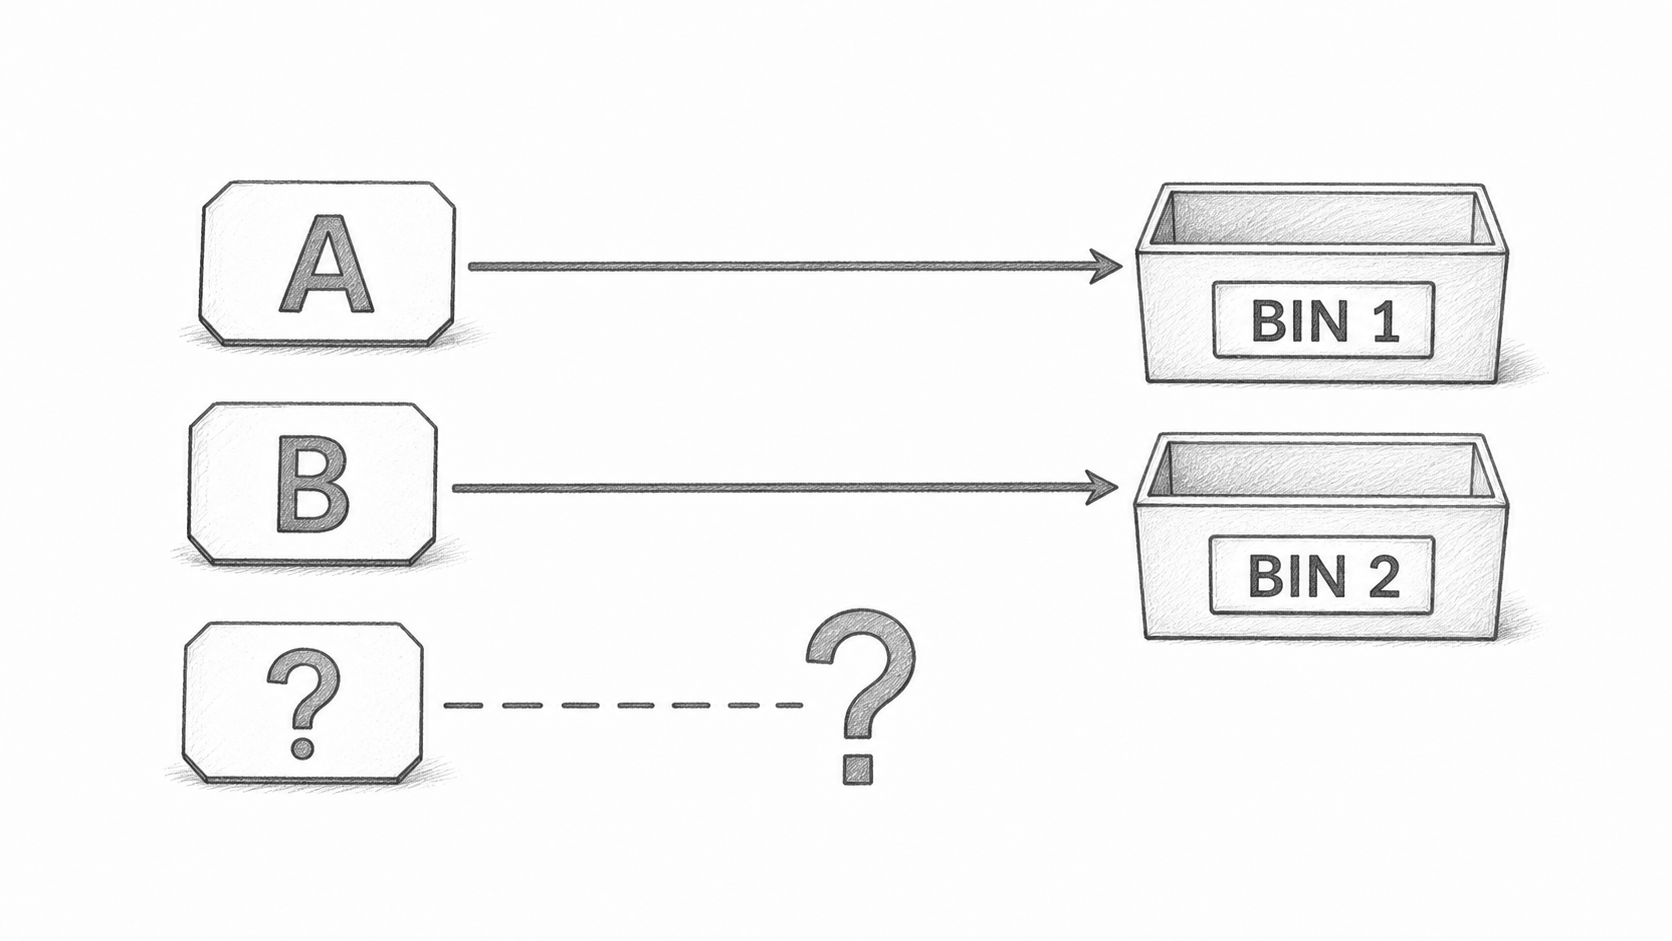
\includegraphics[width=0.98\linewidth,height=0.27\textheight,
 keepaspectratio]{049-token-bin-map-pencil.png}

\small\textit{Alternative text: a graphite pencil drawing maps card A by a
solid arrow to Bin 1 and card B by a solid arrow to Bin 2. A third card marked
with a question mark follows a dashed line to a larger question mark.}
\end{center}

\texttt{LocalIdentityRegistry} owns no reader, keypad, pin, endpoint, timer,
interrupt, bus, clock, storage transport, supply, or moving hardware. It
borrows a live binding array, exactly two 160-byte image slots, and one
160-byte candidate buffer. These caller-owned arrays must outlive the registry
and must not move.

\begin{tabularx}{\linewidth}{@{}l r X@{}}
\toprule
Fixed limit & Value & Meaning\\
\midrule
identity bytes & 10 & 4--10 significant bytes, then canonical zero padding\\
local bindings & 8 & allocation-free compile-time maximum\\
carousel bins & 8 & local metadata, not part of identity equality\\
image slots & 2 & complete supplied images, never an inferred empty directory\\
image bytes & 160 & canonical byte encoding, not a copied C++ struct\\
\bottomrule
\end{tabularx}

\newpage
\section{Read a canonical fixed image}
\begin{center}
% ADK visual: pencil
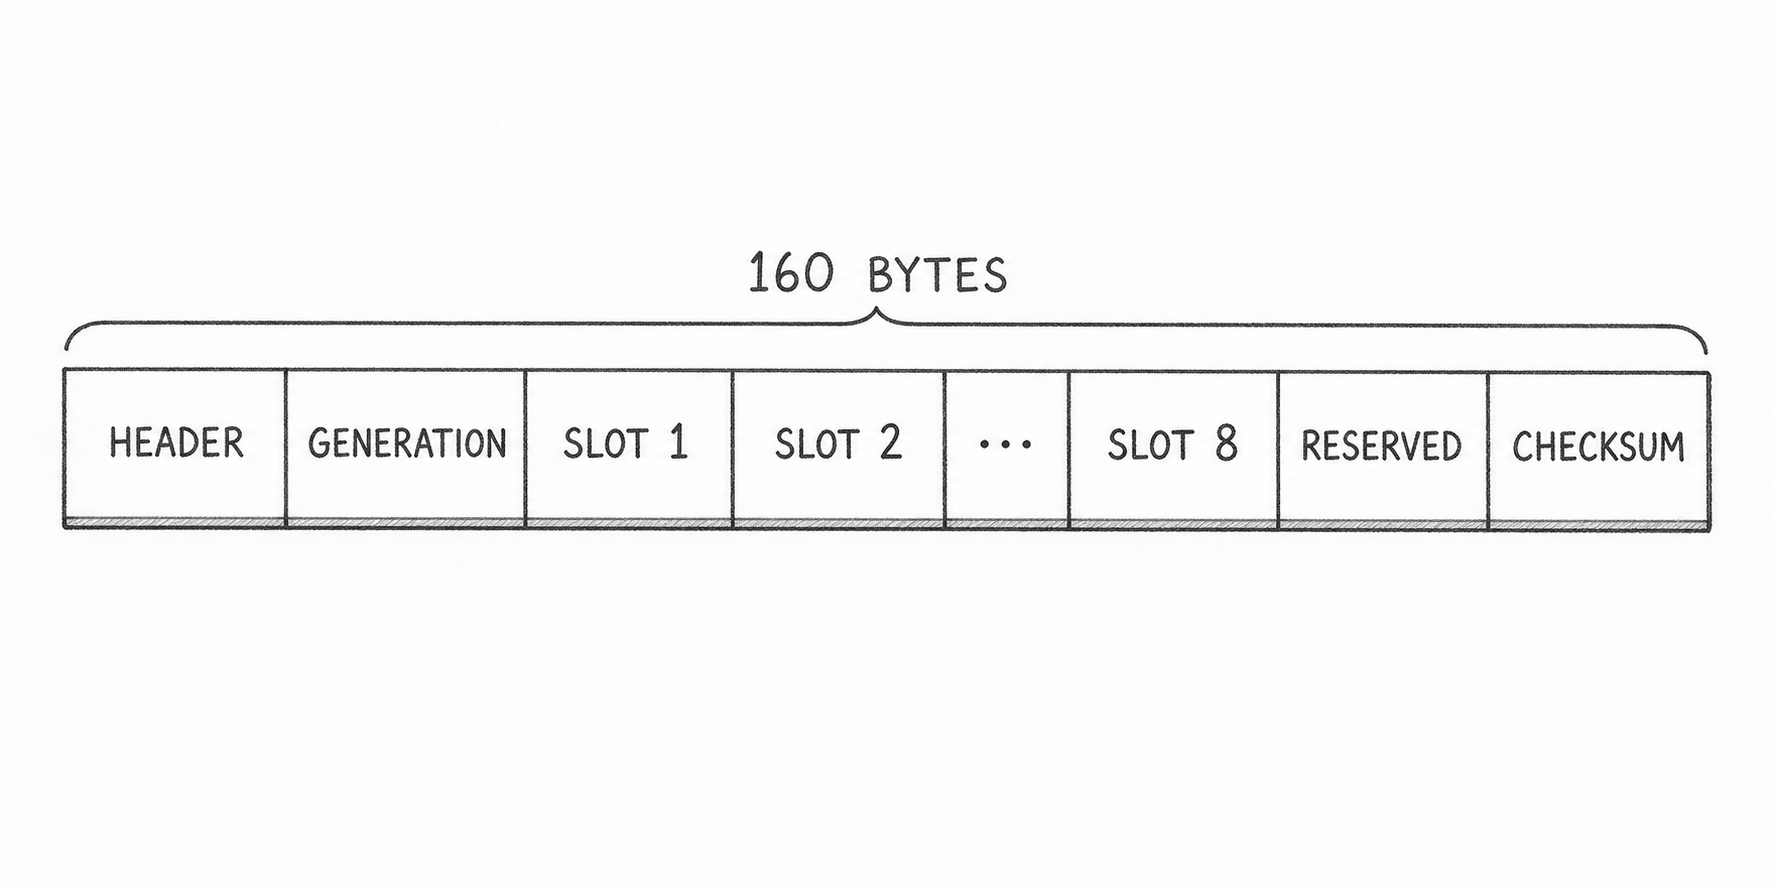
\includegraphics[width=0.98\linewidth,height=0.25\textheight,
 keepaspectratio]{049-fixed-record-anatomy-pencil.png}

\small\textit{Alternative text: a graphite pencil drawing shows one
160-byte horizontal record divided into Header, Generation, Slot 1, Slot 2,
an ellipsis, Slot 8, Reserved, and Checksum regions.}
\end{center}

Multibyte integers are unsigned little-endian. Reserved bytes and unused
entries are zero. CRC-16/CCITT-FALSE detects malformed fixture bytes; it does
not provide authenticity, secrecy, or adversarial integrity.

\begin{tabularx}{\linewidth}{@{}r r X@{}}
\toprule
Offset & Bytes & Canonical meaning\\
\midrule
0 & 2 & magic \texttt{0x4944}\\
2 & 1 & schema version \texttt{1}\\
3 & 1 & flags, exactly zero\\
4 & 2 & encoded length, exactly 160\\
6 & 4 & nonzero registry configuration ID\\
10 & 4 & image generation\\
14 & 1 & binding count, 0--8\\
15 & 1 & reserved zero\\
16 & 128 & eight fixed 16-byte binding entries\\
144 & 14 & reserved zero\\
158 & 2 & checksum over bytes 0--157\\
\bottomrule
\end{tabularx}

Each used entry stores length at \(+0\), ten zero-padded identity bytes at
\(+1\ldots+10\), bin at \(+11\), nonzero revision at \(+12\ldots+13\), and
an entry checksum at \(+14\ldots+15\). All-zero and all-\texttt{0xff}
identifiers are fixture sentinels and are rejected.

\section{Reconstruction worksheet}
\begin{tabularx}{\linewidth}{@{}X X X@{}}
\toprule
Supplied slots & Predict selected result & Observed / interpretation\\
\midrule
generation 4 valid; other erased & generation 4 & \blankline\\[7pt]
generation 4 valid; other corrupt & generation 4 & \blankline\\[7pt]
generations 4 and 5 valid & generation 5 & \blankline\\[7pt]
equal generation, unequal bytes & reject & \blankline\\[7pt]
half-range generation difference & reject ambiguous order & \blankline\\[7pt]
both invalid & fail closed, not empty & \blankline\\
\bottomrule
\end{tabularx}

\newpage
\section{Observe, classify, and bound failures}
\begin{center}
% ADK visual: pencil
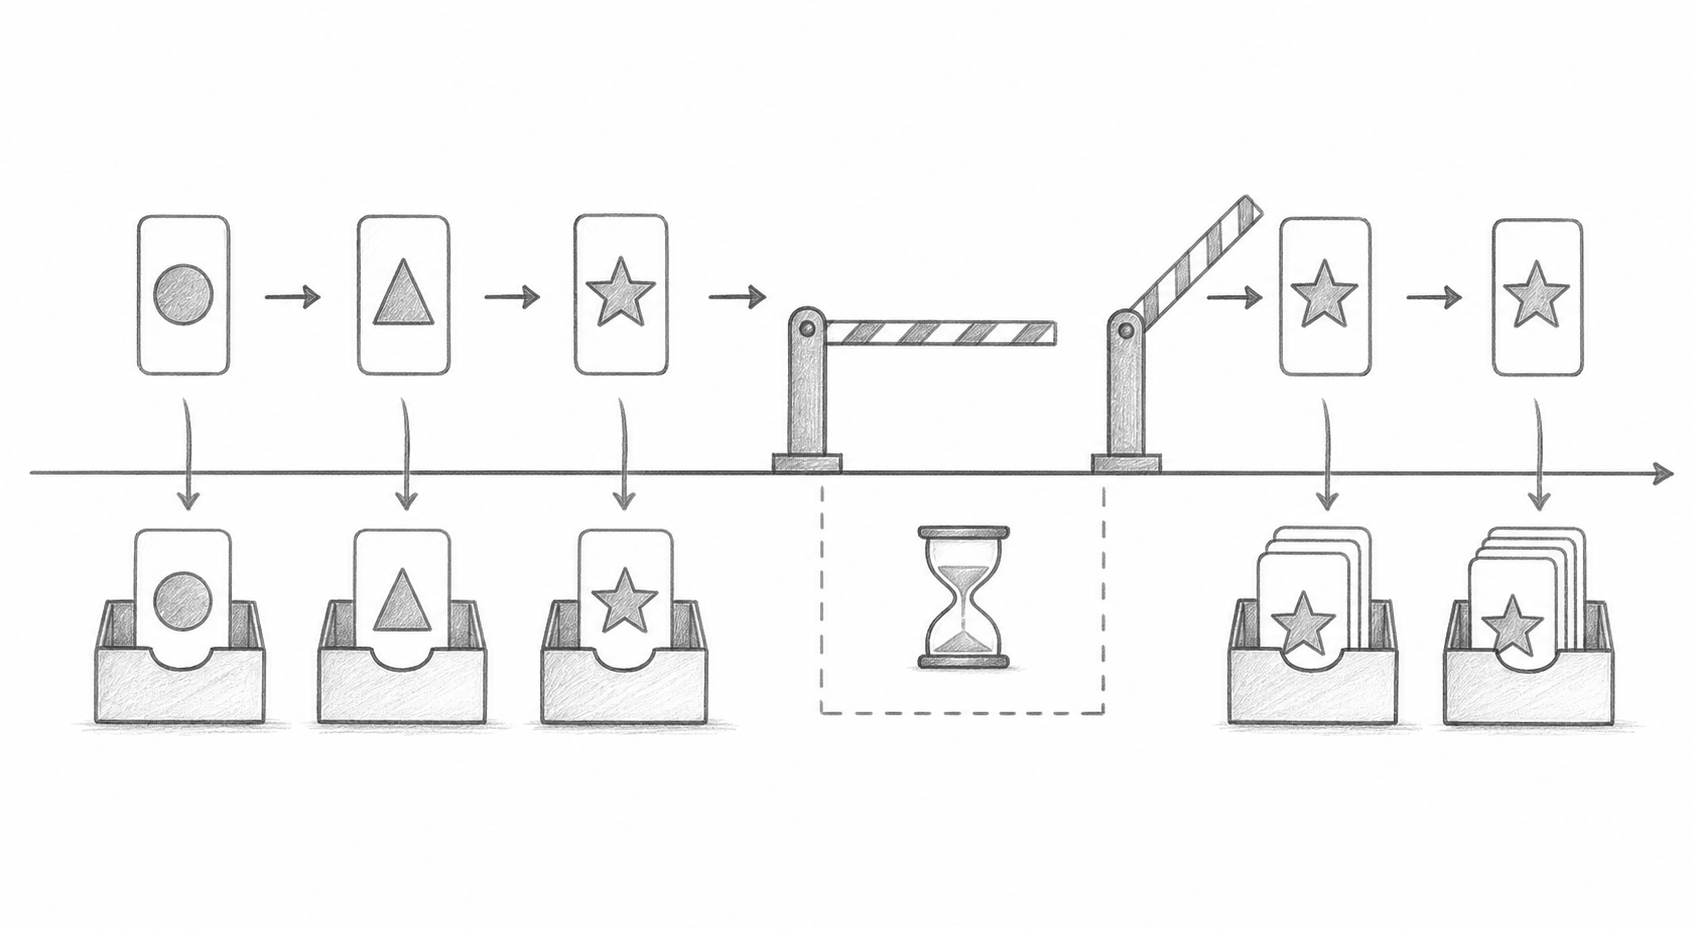
\includegraphics[width=0.98\linewidth,height=0.24\textheight,
 keepaspectratio]{049-lockout-timeline-pencil.png}

\small\textit{Alternative text: a graphite pencil timeline shows circle,
triangle, and star cards above matching single-card bins. A lowered barrier,
an hourglass below the timeline, and then a raised barrier separate those
single cards from two later star cards above bins containing stacked copies.}
\end{center}

Evidence retains source kind, source ID, configuration revision, occurrence
time, sequence, identifier, and complete producer status. Same-domain
sequence deltas \(1\ldots\texttt{INT32\_MAX}\) move forward. Delta zero is an
exact replay only; changed payload at the same sequence is malformed.
\texttt{0x80000000} is ambiguous, and larger deltas regress.

An unknown identifier increments a saturating failure count once per admitted
new sequence. Reaching \texttt{maximumFailures} begins lockout for exactly
\texttt{lockoutDuration}; the exact expiry boundary is usable. A known result
clears failures only after expiry. Structural, source, time, and image faults
take precedence and never increment the count.

\begin{tabularx}{\linewidth}{@{}l X@{}}
\toprule
Condition & Predicted disposition\\
\midrule
identifier matches length and bytes & \texttt{Known}; expose bin and binding revision\\
canonical but unmatched identifier & \texttt{Unknown}; count one new attempt\\
exact same-sequence replay & age may change; no new attempt\\
same sequence with one changed byte & \texttt{Malformed}; preserve accepted history\\
maximum failures reached & \texttt{LockedOut}\\
known identity at exact lockout expiry & \texttt{Known}; clear failure count\\
full table during enrollment & \texttt{DirectoryFull}\\
\bottomrule
\end{tabularx}

\section{Timing worksheet}
\begin{tabularx}{\linewidth}{@{}r r r X@{}}
\toprule
Now & Observed at & Sequence & Prediction / reason\\
\midrule
20 & 20 & 2 & \blankline\\[6pt]
40 & 40 & 4 & \blankline\\[6pt]
40 & 40 & 4 exact replay & \blankline\\[6pt]
91 & 40 & 4 exact replay & \blankline\\[6pt]
40 & 41 & 5 & \blankline\\[6pt]
\texttt{0} & \texttt{0xfffffff0} & next & \blankline\\
\bottomrule
\end{tabularx}

\newpage
\section{Stage enrollment without claiming persistence}
Ordinary observation never enrolls. The transaction keeps the live directory
unchanged until an external coordinator reports exact reconciled evidence.
The caller supplies a nonzero \texttt{instanceEpoch}; initialization rejects
zero, and the value must be caller-unique across every concurrent or
reconstructed registry lifetime so foreign or old candidates cannot become
current. No hidden static counter or object/buffer address supplies that
identity.

\begin{enumerate}
 \item \texttt{previewEnrollment()} validates a fresh unknown identity,
       vacant bin, capacity, lockout state, and base generation.
 \item \texttt{previewExport()} exposes a bounded view of the complete
       canonical candidate image. It is retryable and does not commit.
 \item A future external coordinator may write the inactive durable slot,
       synchronize it, reread it, and validate it.
 \item \texttt{acknowledgeExternalCommit()} validates matching owner,
       generations, operation, slot, view metadata, checksum, bytes, and
       durable status, then installs the candidate atomically.
\end{enumerate}

\lessonbox{\textbf{E0 boundary.} The compile-only replay supplies matching
acknowledgement evidence from caller-owned RAM. It performs no EEPROM, SD,
RFID, SPI, keypad, or filesystem operation and proves no retention,
power-loss survival, wear endurance, or media atomicity.}

\begin{tabularx}{\linewidth}{@{}l X X@{}}
\toprule
Case & Prediction & Observation / interpretation\\
\midrule
known identity & enrollment rejected & \blankline\\[7pt]
occupied bin & enrollment rejected & \blankline\\[7pt]
valid preview, then cancel & no live binding added & \blankline\\[7pt]
foreign, stale, or earlier-epoch candidate & reject without mutation &
\blankline\\[7pt]
negative or mismatched acknowledgement & preserve retryable candidate;
reconciliation required & \blankline\\[7pt]
exact successful acknowledgement & install once, advance generation & \blankline\\[7pt]
byte-identical successful duplicate & idempotent success & \blankline\\
\bottomrule
\end{tabularx}

\section{Replay the eight named frames}
Use
\href{https://github.com/spincyc/adk/blob/main/examples/Lesson049LocalIdentityRegistry/Lesson049LocalIdentityRegistry.ino}
{the Lesson 049 compile-only sketch}. Predict before inspecting each volatile
result cell. Its flow is acquire, configure, start; then observe, decide, and
record. Recording changes only fixture-owned memory.

\begin{tabularx}{\linewidth}{@{}c l X X@{}}
\toprule
Frame & Scripted action & Prediction & Result / interpretation\\
\midrule
1 & observe token A & unknown & \blankline\\[5pt]
2 & enroll A at bin 2 & commit; generation advances & \blankline\\[5pt]
3 & observe A & known bin 2 & \blankline\\[5pt]
4 & observe token B & unknown; failure count 1 & \blankline\\[5pt]
5 & exact replay B & no second failure & \blankline\\[5pt]
6 & preview then cancel token C & directory unchanged & \blankline\\[5pt]
7 & observe B & lockout begins & \blankline\\[5pt]
8 & observe C during lockout & locked out & \blankline\\
\bottomrule
\end{tabularx}

\newpage
\section{Separate acquisition, record result, and safe state}
\begin{tabularx}{\linewidth}{@{}>{\bfseries}l X X@{}}
\toprule
Stage & Predict & Observe and interpret\\
\midrule
Acquire & validate config, extents, non-overlap, and both images & status:
\blankline\\[10pt]
Observe & admit one complete synthetic identity & sequence/disposition:
\blankline\\[10pt]
Reset & clear observation, lockout, and ordinary pending work; retain committed
directory & snapshot: \blankline\\[10pt]
Shutdown & publish inactive lifecycle; preserve required reconciliation &
status: \blankline\\
\bottomrule
\end{tabularx}

Initialization proves only that a pure object accepted its configuration and
borrowed memory. Reset and shutdown prove only software state. None proves an
RFID transaction, keypad level, storage write, inactive pin, safe voltage, or
power-removal behavior.

\section{Resource record}
\begin{tabularx}{\linewidth}{@{}l X@{}}
\toprule
Gate & Record\\
\midrule
\texttt{sizeof(LocalIdentityRegistry)} & measured: 121 bytes;
hard ceiling: 128 bytes\\[6pt]
complete Mega sketch & flash: 7,026 bytes (limit 16,384);
static SRAM: 1,113 bytes (limit 1,280)\\[6pt]
caller-owned buffers & two 160-byte images, one 160-byte candidate, and eight
bounded live bindings included in whole-sketch SRAM\\[6pt]
runtime reserve & Mega SRAM: 8,192 bytes; 7,079 bytes remain after 1,113
static bytes; reserving 512 bytes for stack/ISR leaves 6,567 bytes, exceeding
the required 768-byte margin\\[6pt]
owned resources & no heap, pins, ADC, timers, interrupts, buses, endpoints,
supplies, persistent medium, or moving hardware\\[6pt]
host evidence & deterministic, corruption, rollover, lifecycle, sanitizer,
and AVR size gates: passed for this host-verified E0 publication\\
\bottomrule
\end{tabularx}

These measured cells are compile and layout evidence for the tested
publication. They are not bench evidence.

\section{Diagnose fixed-record failures}
\begin{enumerate}
 \item Flip each covered byte without updating its checksum. Predict image or
       entry rejection and no partial live-table mutation.
 \item Change identity padding beyond its declared length. Predict
       noncanonical-image rejection even when significant bytes match.
 \item Supply one valid and one corrupt slot. Predict deterministic recovery
       from the valid slot; do not call it a durable-media recovery test.
 \item Interrupt the modeled handoff with indeterminate acknowledgement.
       Predict that new work remains latched off until exact reconciliation.
 \item Reset or shut down during ordinary pending work. Contrast that result
       with a reconciliation-required transaction, which must not disappear.
\end{enumerate}

\newpage
\small
\section{Blank E1 reader, keypad, and media acceptance record}
\textbf{Leave every field blank until separately qualified powered and media
work is performed and reviewed. E1 authorizes no motor, servo, or moving load.}

\begin{tabularx}{\linewidth}{@{}l X@{}}
\toprule
Required field & Bench record\\
\midrule
board revision / tested commit & \blankline\\[5pt]
exact RFID reader and token markings & \blankline\\[5pt]
exact keypad and home/stop specimen markings & \blankline\\[5pt]
exact nonvolatile medium / adapter / revision & \blankline\\[5pt]
primary electrical and media references & \blankline\\[5pt]
supply / logic levels / pin and resource map & \blankline\\[5pt]
instrument / tool version & \blankline\\[5pt]
resource-acquisition and rollback prediction & \blankline\\[5pt]
resource-acquisition and rollback observation & \blankline\\[5pt]
non-Serial test point prediction / observation & \blankline\\[5pt]
safe-state prediction / observation & \blankline\\[5pt]
write / synchronize / reread measurement & \blankline\\[5pt]
power-removal and restart result & \blankline\\[5pt]
interpretation / reviewer / date & \blankline\\
\bottomrule
\end{tabularx}

\section{Claim boundary and evidence links}
No retail kit name establishes a reader chip, protocol, voltage, pinout,
keypad topology, or storage technology. UID-shaped bytes do not become a
credential. Checksums do not become cryptographic integrity. Supplied RAM
images do not become persistent media. Physical position and dispensing
remain unknown; restrained actuator and gate work belongs to E2.

\begin{itemize}
 \item \href{https://github.com/spincyc/adk/blob/main/src/local_identity_registry.h}
       {Public interface}
 \item \href{https://github.com/spincyc/adk/blob/main/tests/test_local_identity_registry.cpp}
       {Deterministic host tests}
 \item \href{https://github.com/spincyc/adk/blob/main/examples/Lesson049LocalIdentityRegistry/Lesson049LocalIdentityRegistry.ino}
       {Compile-only synthetic-record replay}
 \item \href{https://github.com/spincyc/adk/blob/main/docs/design/LESSONS_049_051_PARTS_CAROUSEL_PLAN.md}
       {Reviewed design and open E1/E2 gates}
\end{itemize}

The searchable HTML lesson is the hardware-independent accessible route.
This untagged print edition makes no PDF/UA, powered-reader, persistent-media,
motion, or physical-acceptance claim.
\end{document}
